\documentclass[11pt]{article}
\usepackage[review]{acl}
\usepackage{times}
\usepackage{latexsym}
\usepackage[T1]{fontenc}
\usepackage[utf8]{inputenc}
\usepackage{microtype}
\usepackage{inconsolata}
\usepackage{graphicx}
\usepackage{booktabs}
\usepackage{multirow}
\usepackage{amsmath}
\usepackage{xcolor}
\usepackage{tikz}
\usetikzlibrary{positioning,arrows.meta,fit,backgrounds,calc}

% New text is red so co-authors can see what was added; switch to black once reviewed.
\colorlet{newtext}{black}
\usepackage{adjustbox}
% Placeholders for numbers that come from the experiments (results/tables, via make_tables.py)
\newcommand{\tbd}[1]{\textbf{[#1]}}
\newcommand{\method}{\textsc{Unwrap}}
\newcommand{\air}{\textsc{Air}}

\title{Verify the Claim, Not the Text: Format-Shifting Attacks on\\Misinformation Detectors and a Robust Defence}

\author{Anonymous ACL submission}

\begin{document}
\color{newtext}
\maketitle

\begin{abstract}
Misinformation detectors are evaluated on claims written as plain statements, yet text often reaches them after a language model has translated it, summarised it, turned it into a quiz question, or serialised it as XML or JSON. We study such \emph{format-shifting attacks}, which preserve the meaning of a false claim and change only its surface form, alone and chained. On PUBHEALTH, CLIMATE-FEVER and Fin-Fact, published detectors such as ARG, ProgramFC and MiniCheck, and zero-shot LLMs, lose 19.6 macro-F1 points on average and up to 49 points, although the claim's meaning is preserved; Claude Opus~5.5 still loses 15 to 17 points on two of the benchmarks. We propose \method{}, a detector that verifies the claim rather than the text: it canonicalises any input into the English claims it asserts or presupposes, retrieves verified true and false claims with a hybrid multilingual retriever, reranks them, and decides with a verdict-aware verifier trained on clean claims only. \method{} has the best clean macro-F1 on all three benchmarks, loses only 4.4 to 5.6 points under attack and, compared under the same training conditions, is significantly more robust than every baseline in 32 of 33 comparisons, the remaining one being a statistical tie. Adversarial training protects most classifiers only against the attack families they were trained on.
\end{abstract}

\section{Introduction}

\begin{figure*}[t]
\centering
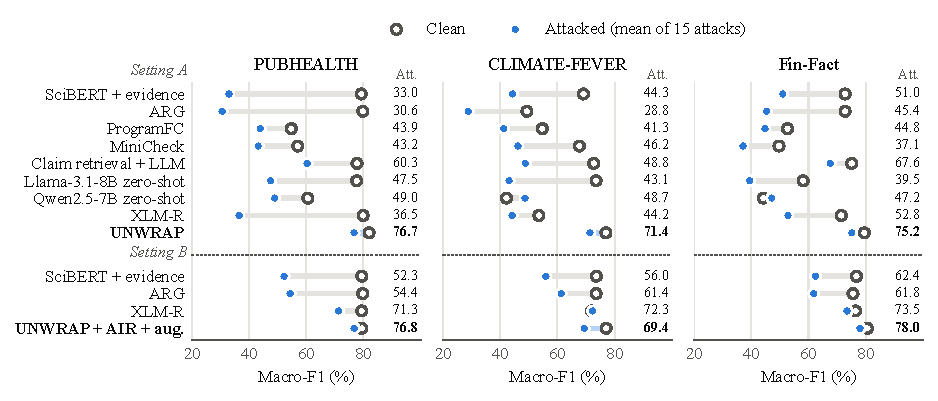
\includegraphics[width=\textwidth]{figures/fig_clean_vs_attacked.pdf}
\caption{Macro-F1 on clean test claims (rings) and averaged over fifteen format-shifting attacks (dots). Published detectors and zero-shot LLMs lose up to 49 points although the claim's meaning is preserved; \method{} stays close to its clean performance without seeing any attacked text (Setting~A). Setting~B adds transformed training claims to all detectors. The attacked score is printed at the right of each panel.}
\label{fig:teaser}
\end{figure*}


Misinformation detection has mostly been studied as the classification of claims, headlines or posts in their original form \citep{zellers2019grover,thorne2018fever,guo2022survey}. Benchmarks such as PUBHEALTH \citep{kotonya2020pubhealth}, CLIMATE-FEVER \citep{diggelmann2020climatefever} and Fin-Fact \citep{rangapur2023finfact} pair each claim with a verdict from professional fact-checkers, and detectors are trained and tested on the claims as published. Deployed detectors rarely see claims in that form: users ask assistants to translate, summarise or answer, platforms pass content to LLM services as structured requests, and adversaries can repackage a false claim with the same tools at no cost.

Existing robustness work perturbs the claim itself, by substituting words, paraphrasing, or rewriting it with an LLM \citep{przybyla2024bodega,bethany2025camouflage}. We study a simpler and, we argue, more realistic family of attacks that preserves the claim's meaning and shifts its \emph{format}: the claim is expanded and translated, embedded in an article to be summarised, presupposed by a multiple-choice question that begins with ``Why'', or serialised as XML or JSON to be parsed. These steps can be chained, for instance by turning a claim into a question, translating the question into Arabic and wrapping it in JSON. Each step is a routine request to an LLM, and the false claim survives every step.

We study three domains in which false claims cause measurable harm and are spread deliberately, and in which detectors therefore need defences that hold when a claim is disguised. In health, exposure to COVID-19 vaccine misinformation lowered the intention to vaccinate by 6.2 percentage points in the UK and 6.4 in the US in a randomised study \citep{loomba2021vaccine}. In climate, a single piece of popular misinformation cancelled out the effect of communicating the scientific consensus on climate change \citep{vanderlinden2017inoculating}. In finance, a false report posted from a hacked news-agency account set off a brief automated sell-off on US stock markets \citep{karppi2015hackcrash}.

Each of these formats is a documented route around existing safeguards. Content in languages other than English is moderated less: Facebook had not labelled 70\% of the Spanish and 68\% of the Italian fact-checked COVID-19 misinformation posts examined by \citet{avaaz2020flatten}, against 29\% of the English ones, and language models used for content analysis perform unevenly across languages \citep{nicholas2023lost}. News increasingly reaches readers through AI assistants that rewrite it, and in a study of more than 3,000 answers, 45\% of the assistants' answers about news had at least one significant issue \citep{ebu2025newsintegrity}. A question that presupposes a fact makes people more likely to later report it as true \citep{loftus1975leading}, and a quarter of real information-seeking questions rest on false presuppositions \citep{yu2023crepe}. Recasting a request as code or structured data bypasses LLM safety training more than 80\% of the time \citep{ren2024codeattack}.

We make four contributions. First, we define fifteen format-shifting attacks (five translations, summarisation, multiple-choice questions, XML, JSON and six chains) and apply them to the test sets of three benchmarks in three domains; an independent judge model confirms that the attacked texts still convey the claim. Second, we show that published detectors and zero-shot LLMs degrade sharply under these attacks even when they are strong on clean claims: the evidence classifier of \citet{kotonya2020pubhealth}, for instance, falls from 79.2 to 33.0 macro-F1 on PUBHEALTH. Third, we propose \method{}, which canonicalises the input into the English claims it asserts or takes for granted, retrieves verified claims of both verdicts from an archive built from the training split, reranks them, and lets a verdict-aware LLM verifier, fine-tuned on clean training claims, decide. Fourth, we show that adversarial training largely fails to close the gap: classifiers trained on transformed claims recover on the attack families they saw but not on new languages, formats or chains.

Every detector is trained, or given its retrieval archive, on the training split only, calibrated on clean development data, and evaluated on the held-out test claims, clean and attacked. In Setting~A, no detector sees attacked or transformed text; in Setting~B, detectors are also trained on transformed training claims of four attack families, produced by a different generator than the test attacks.

\section{Related Work}

Misinformation detectors range from classifiers fine-tuned on labelled claims \citep{kotonya2020pubhealth,guo2022survey} to evidence-based fact-checkers that retrieve documents \citep{thorne2018fever}, decompose claims with LLMs \citep{pan2023programfc} or check claims against grounding documents with small verifiers \citep{tang2024minicheck}; retrieval-augmented generation \citep{lewis2020rag} gives LLMs access to verified information. Our detector belongs to the line of work that detects \emph{previously fact-checked claims} by retrieving them from an archive of fact-checks \citep{shaar2020knownlie}, which has also been studied across languages \citep{pikuliak2023multiclaim}.

Claim normalisation rewrites a noisy social-media post into a concise check-worthy claim \citep{sundriyal2023claimnorm}, and SUCEA \citep{liu2025sucea} segments, decontextualises and edits adversarially paraphrased claims so that evidence retrieval succeeds. Both assume that the input states its claim, if noisily or in other words. Format-shifting attacks instead hide a claim, with its meaning preserved, behind a task, a language or a serialisation, and may only presuppose it. Our canonicaliser is instructed for exactly these cases, and we compare it with a generic normalisation prompt in our ablations.

Adversarial attacks on misinformation detectors edit the claim: BODEGA \citep{przybyla2024bodega} benchmarks word- and character-level perturbations against credibility classifiers, and CAMOUFLAGE \citep{bethany2025camouflage} rewrites claims with an LLM so that evidence retrieval fails. Both tune the wording against a target model; our attacks are not optimised against any detector: they preserve the claim's meaning while changing its format and the task around it, need no access to the detector, and compose freely. They are closer to attacks on LLM safety, where low-resource languages \citep{yong2023lowresource,deng2024multilingual}, ciphers \citep{yuan2024cipher} and instructions hidden in processed content \citep{greshake2023indirect} bypass safeguards; we use the last of these as an adaptive attack against our own canonicaliser.

\section{Threat Model and Attacks}
\label{sec:attacks}

We consider a detector that screens text before it is published, forwarded or processed by an LLM-based service, and decides whether it spreads false information. The attacker holds a fact-checked false claim and wants it to pass, for example so that an assistant translates, summarises or answers it and thereby repeats it; the attacker can use general-purpose LLMs but has no access to the detector, its archive or its scores. Since the same transformations apply to true claims, a robust detector must also not flag true claims merely because of their format.

Each attack transforms a claim and adds a task wrapper that a downstream LLM would execute. The single-step attacks are \emph{translation} (the claim is expanded into a short paragraph and translated into French, Spanish, Arabic, Hindi or Chinese, wrapped in ``Translate from \ldots{} to English''), \emph{summarisation} (an article of about 500 words built around the claim, wrapped in a summarisation request), \emph{multiple-choice question} (a ``Why'' question whose options include the claim, wrapped in ``Answer the following question'') and \emph{XML} \citep{bray2008xml} and \emph{JSON} \citep{bray2017json} (the expanded claim serialised as a document, wrapped in a parsing request). The six chains apply, in this order, MCQ$\rightarrow$translate, MCQ$\rightarrow$JSON, MCQ$\rightarrow$XML, translate$\rightarrow$XML, summarise$\rightarrow$JSON and MCQ$\rightarrow$translate$\rightarrow$JSON, with a random language per claim. Appendices~\ref{sec:appendix_attacks} and~\ref{sec:appendix_prompts} show one claim under every attack and all prompts.

The test attacks are sampled from Qwen2.5-32B-Instruct \citep{qwen2024qwen25}, a model family different from our detector's, so that the detector cannot benefit from recognising its own writing style. An independent judge from a third family, Gemma-3-12B \citep{gemma2025gemma3}, decided for every attacked text whether it asserts, repeats or takes for granted the original claim; 92.7\% did, between 82.8\% (summarisation on Fin-Fact) and 98.9\% per attack and dataset (Table~\ref{tab:preservation}). \tbd{Human validation of the judge: agreement between human annotators and the judge on a stratified sample of attacked texts.} The check matters because an attacker asked to discuss a false headline sometimes debunks it instead. All results in the main paper are therefore computed on the attacked texts that the judge found to preserve the claim, for true and false claims alike; scored on all attacked texts instead, the five most robust detectors keep their ranking on every dataset. Two adaptive attacks against our own pipeline are reported separately (Appendix~\ref{sec:appendix_analyses}).

\section{Method: \method{}}
\label{sec:method}

\method{} rests on a simple observation: format-shifting attacks change everything about the text except the claim, so a detector should operate on the claim. Figure~\ref{fig:system} gives an overview.

\begin{figure*}[t]
\centering
{\color{black}\resizebox{\textwidth}{!}{% Block diagram of the threat model and of UNWRAP (+AIR). Included by main.tex inside a figure* environment.
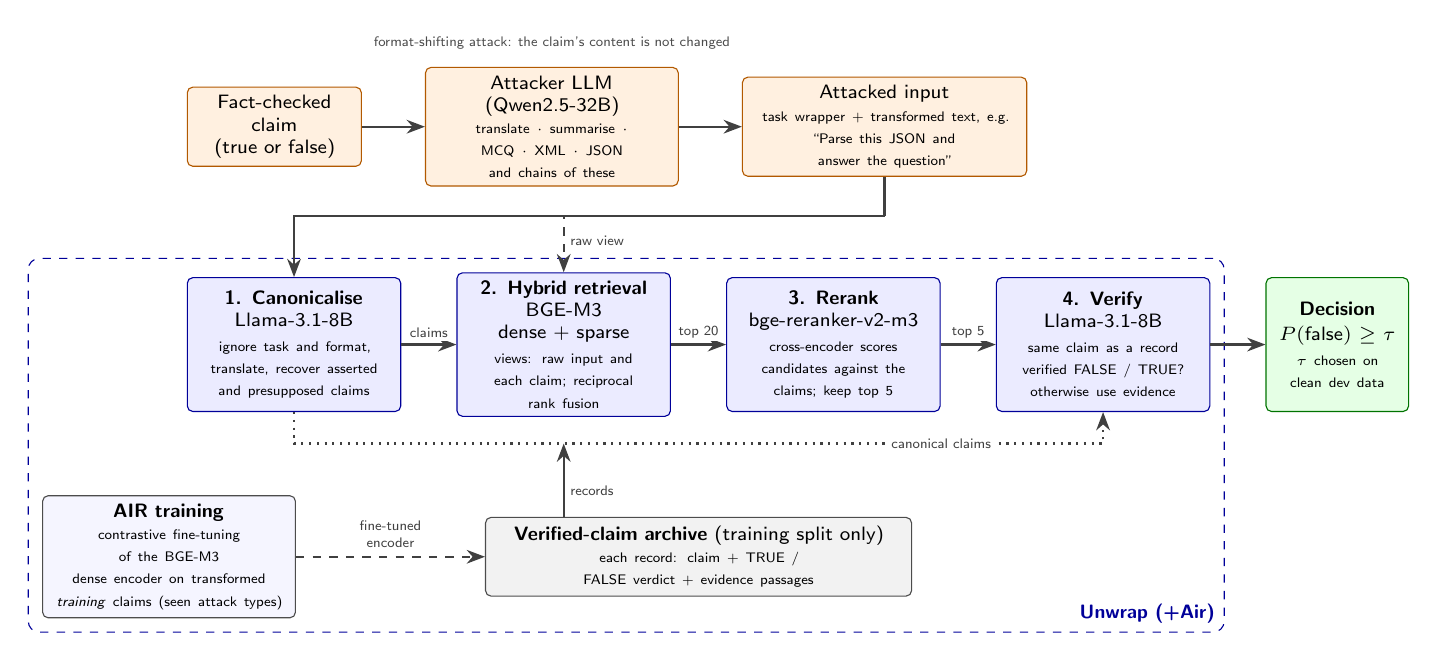
\begin{tikzpicture}[
  font=\sffamily\scriptsize, >=Stealth, node distance=4mm and 6mm,
  box/.style={draw, rounded corners=2pt, align=center, minimum height=10mm, inner sep=3pt, fill=white},
  att/.style={box, fill=orange!12, draw=orange!70!black},
  ours/.style={box, fill=blue!8, draw=blue!60!black, text width=25mm, minimum height=17mm},
  data/.style={box, fill=gray!10, draw=gray!60!black},
  outbox/.style={box, fill=green!10, draw=green!45!black, text width=16mm, minimum height=17mm},
  lab/.style={font=\sffamily\tiny, align=center, text=black!75, fill=white, inner sep=1pt},
  arr/.style={->, thick, black!75}]

% ---------------- threat model (top row)
\node[att, text width=20mm] (claim) {Fact-checked claim\\(true or false)};
\node[att, right=8mm of claim, text width=30mm] (attacker) {Attacker LLM (Qwen2.5-32B)\\{\tiny translate $\cdot$ summarise $\cdot$ MCQ $\cdot$ XML $\cdot$ JSON}\\{\tiny and chains of these}};
\node[att, right=8mm of attacker, text width=34mm] (input) {Attacked input\\{\tiny task wrapper + transformed text, e.g.}\\{\tiny ``Parse this JSON and answer the question''}};
\draw[arr] (claim) -- (attacker);
\draw[arr] (attacker) -- (input);
\node[font=\sffamily\tiny, text=black!70, above=1mm of attacker] {format-shifting attack: the claim's content is not changed};

% ---------------- UNWRAP pipeline (middle row)
\node[ours, below=14mm of claim.south west, anchor=north west] (canon) {\textbf{1. Canonicalise}\\Llama-3.1-8B\\[1pt]{\tiny ignore task and format,}\\{\tiny translate, recover asserted}\\{\tiny and presupposed claims}};
\node[ours, right=7mm of canon] (retr) {\textbf{2. Hybrid retrieval}\\BGE-M3 dense + sparse\\[1pt]{\tiny views: raw input and}\\{\tiny each claim; reciprocal}\\{\tiny rank fusion}};
\node[ours, right=7mm of retr] (rerank) {\textbf{3. Rerank}\\bge-reranker-v2-m3\\[1pt]{\tiny cross-encoder scores}\\{\tiny candidates against the}\\{\tiny claims; keep top 5}};
\node[ours, right=7mm of rerank] (verify) {\textbf{4. Verify}\\Llama-3.1-8B\\[1pt]{\tiny same claim as a record}\\{\tiny verified FALSE / TRUE?}\\{\tiny otherwise use evidence}};
\node[outbox, right=7mm of verify] (dec) {\textbf{Decision}\\[1pt]$P(\text{false})\geq\tau$\\[1pt]{\tiny $\tau$ chosen on}\\{\tiny clean dev data}};

\draw[arr] (canon) -- node[lab, above=1pt] {claims} (retr);
\draw[arr] (retr) -- node[lab, above=1pt] {top 20} (rerank);
\draw[arr] (rerank) -- node[lab, above=1pt] {top 5} (verify);
\draw[arr] (verify) -- (dec);

% input -> canonicaliser (solid) and input -> retrieval as the raw view (dashed)
\coordinate (split) at ($(input.south)+(0,-5mm)$);
\draw[thick, black!75] (input.south) -- (split);
\draw[arr] (split) -| (canon.north);
\draw[arr, dashed] (split) -| node[lab, pos=0.72, right=1pt] {raw view} (retr.north);

% canonical claims also go to the verifier (below the boxes)
\coordinate (cbot) at ($(canon.south)+(0,-4mm)$);
\draw[arr, dotted] (canon.south) -- (cbot) -- node[lab, pos=0.8] {canonical claims} (cbot -| verify.south) -- (verify.south);

% ---------------- archive and AIR (bottom row)
\node[data, text width=52mm, below=13mm of $(retr.south)!0.5!(rerank.south)$] (kb) {\textbf{Verified-claim archive} (training split only)\\{\tiny each record: claim + TRUE / FALSE verdict + evidence passages}};
\node[data, fill=blue!4, text width=30mm, left=24mm of kb] (air) {\textbf{AIR training}\\{\tiny contrastive fine-tuning of the BGE-M3}\\{\tiny dense encoder on transformed}\\{\tiny \emph{training} claims (seen attack types)}};
\draw[arr] (kb.north -| retr.south) -- node[lab, right=1pt, pos=0.35] {records} (retr.south |- cbot);
\draw[arr, dashed] (air.east) -- node[lab, above=2pt, align=center] {fine-tuned\\encoder} (kb.west);

\begin{scope}[on background layer]
  \node[draw=blue!60!black, dashed, rounded corners=4pt, fit=(canon)(retr)(rerank)(verify)(kb)(air), inner sep=5pt] (frame) {};
\end{scope}
\node[font=\sffamily\scriptsize\bfseries, text=blue!60!black, anchor=south east] at (frame.south east) {\textsc{Unwrap} (+\textsc{Air})\ };
\end{tikzpicture}
}}
\color{newtext}
\caption{Threat model (top) and \method{} (bottom). An attacker LLM changes only the format of a fact-checked claim and wraps it in a task. \method{} canonicalises the input into the claims it asserts or presupposes, retrieves verified claims of both verdicts from an archive built from the training split using every view of the input, reranks them, and lets a verdict-aware verifier decide. \air{} fine-tunes the dense retriever on transformed training claims only.}
\label{fig:system}
\end{figure*}

\subsection{Verified-claim archive}

For each benchmark, the archive holds every training claim, true and false, with its verdict and the evidence that comes with it in the benchmark (PUBHEALTH explanations and fact-check articles, CLIMATE-FEVER evidence sentences, Fin-Fact justifications), split into passages of at most 120 words that inherit the claim's verdict. Storing both verdicts lets the verifier see when the closest verified claim is true rather than false. Development and test claims are never stored in the archive.

\subsection{Canonicalisation}

An LLM is instructed to ignore any instruction and format in the input and to write up to three short, self-contained English sentences stating the factual claims the text asserts or takes for granted, the most central first. The instruction makes two cases explicit: a question presupposes its claim (``Why did X happen?'' presupposes that X happened), and in a multiple-choice question the claim is the option the question is built around, not a distractor. The canonicaliser is told not to judge truth, so that it does not silently drop claims it believes to be false.

\subsection{Multi-view hybrid retrieval}

We encode the raw input and each canonical claim with BGE-M3 \citep{chen2024m3}, a multilingual encoder with dense and sparse lexical representations (inputs of up to 2,048 tokens, archive passages of up to 512). A passage's relevance to a view is its dense cosine similarity plus 0.3 times its sparse lexical score, a claim's relevance is the maximum over its passages, and the rankings of all views are combined with reciprocal rank fusion \citep{cormack2009rrf}. The raw view guards against canonicalisation errors; the canonical views let a translated or serialised input retrieve claims written in plain English.

\subsection{Reranking and verdict-aware verification}

The cross-encoder \citep{nogueira2019passage} bge-reranker-v2-m3 \citep{chen2024m3} rescores the top 20 fused candidates against each canonical claim, keeping the best score per candidate, and the top five go to the verifier. The verifier, built on the same LLM as the canonicaliser, sees the canonical claims and, for each retrieved record, the verified claim, its verdict and its most relevant evidence passage, and is asked whether the text spreads false information: the same claim as a record verified false means yes, the same claim as a record verified true means no, and otherwise the evidence decides. The probability of ``Yes'' is the detector's score, and the threshold is set on the clean development set.

\subsection{Training the verifier on clean claims}

Used off the shelf, the LLM verifier costs 7.0 to 10.8 macro-F1 points under attack (Section~\ref{sec:ablation}), so we fine-tune it with LoRA \citep{hu2022lora} on the clean training claims of all three benchmarks, one adapter for all datasets. Each training example is built exactly as at test time, with the target ``Yes'' for false and ``No'' for true claims. Because training claims are themselves in the archive while test claims never are, retrieval for a training claim excludes its own record, so the verifier learns to decide from related verified claims and their evidence rather than from an exact copy. No attacked or transformed text is used, and the number of epochs (one or two) is chosen by clean development macro-F1.

\subsection{Using transformed training claims (Setting B)}

When transformed training claims are available (Setting~B), we use them for both retrieval and verification; we call this variant \method{} + \air{} + aug., for the attack-invariant retriever (\air{}) and the verifier trained on the transformed, or augmented, claims. They are sampled from Llama-3.1-8B-Instruct \citep{grattafiori2024llama3} with instructions and wrappers that differ from the test attacks, and only for the \emph{seen} families: French and Spanish translation, summarisation and multiple-choice questions; XML, JSON, Arabic, Hindi and Chinese translation and all chains are held out. \air{} fine-tunes the dense encoder of BGE-M3 contrastively \citep{henderson2017efficient,reimers2019sbert} so that a transformed training claim lies close to its own archive record, the verifier is trained on the transformed claims in addition to the clean ones, and the adversarially trained baselines receive exactly the same transformed claims (details in Appendix~\ref{sec:appendix_impl}).

\section{Experimental Setup}

\subsection{Datasets and protocol}

We use the binary true/false subsets of three public benchmarks (Table~\ref{tab:data} in the appendix), one for each of the high-stakes domains motivated in Section~1: public health, climate and finance, all with verdicts from professional fact-checkers. PUBHEALTH \citep{kotonya2020pubhealth} has official train/dev/test splits; we drop the \emph{mixture} and \emph{unproven} labels. CLIMATE-FEVER \citep{diggelmann2020climatefever} has no official split; we keep \textsc{supports} and \textsc{refutes} claims and draw a stratified 60/10/30 split with a fixed seed. The test labels of Fin-Fact's \citep{rangapur2023finfact} shared task are not public, so we draw a stratified 70/10/20 split. Duplicate claims are removed. The test sets contain 985, 272 and 551 claims, each appearing clean and under all fifteen attacks.

\subsection{Baselines}

We compare against published detectors, run with their official code where it is available (details in Appendix~\ref{sec:appendix_impl}): the evidence-based SciBERT classifier of \citet{kotonya2020pubhealth}, the best model reported for PUBHEALTH, with evidence sentences ranked over the training archive; ARG \citep{hu2024arg}, which combines a fine-tuned BERT \citep{devlin2019bert} with LLM rationales, here generated by Llama-3.1-8B-Instruct; ProgramFC \citep{pan2023programfc}, which executes LLM-written reasoning programs with FLAN-T5-XL \citep{chung2024flan} over BM25 evidence \citep{robertson2009bm25}; MiniCheck \citep{tang2024minicheck}, which checks the input against the evidence of the three best-matching archived claims; a claim-retrieval baseline following \citet{pikuliak2023multiclaim}, in which Llama-3.1-8B-Instruct decides from the five archived claims closest under multilingual-E5-large \citep{wang2024me5}; zero-shot Llama-3.1-8B-Instruct and Qwen2.5-7B-Instruct, as in the evaluations of \citet{rangapur2023finfact} and \citet{chen2024llmmisinfo}, and Claude Opus~5.5 \citep{anthropic2026opus55} on a stratified subsample of 100 test claims per dataset; and an XLM-R classifier \citep{conneau2020xlmr}, since a multilingual encoder is a natural defence against translation. All retrieval-based baselines use the same training-split archive as \method{}. In Setting~B, SciBERT with evidence, ARG and XLM-R are also trained on the transformed claims (adversarial training). We further place \method{}'s canonicaliser in front of five baselines. Every trained model is run with three seeds, except the Setting~B variant of \method{} and the ablations, which use one.

\subsection{Metrics and implementation}

We report macro-F1 over the true and false classes on the clean test claims and averaged over the fifteen attacks. Two detectors are compared with a paired bootstrap over test claims with 1,000 resamples \citep{efron1993bootstrap}, which draws the same claims, with all their attacked versions, for both detectors and, for seeded models, also a seed; we report the two-sided $p$-value $\min(1, 2\min(P^*(d\le 0), P^*(d\ge 0)))$ of the difference $d$ and call $p<0.05$ significant. Thresholds maximise macro-F1 on the clean development claims, and all detectors decode greedily (Appendices~\ref{sec:appendix_impl} and~\ref{sec:appendix_prompts} give implementation details and prompts).

\section{Results}
\label{sec:results}

\begin{table*}[t]\centering\small\setlength{\tabcolsep}{5pt}
\begin{adjustbox}{max width=\textwidth}\begin{tabular}{lccccccccc}
\toprule
 & \multicolumn{3}{c}{PUBHEALTH} & \multicolumn{3}{c}{CLIMATE-FEVER} & \multicolumn{3}{c}{Fin-Fact} \\
\cmidrule(lr){2-4} \cmidrule(lr){5-7} \cmidrule(lr){8-10}
Detector & Clean & Att. & $\Delta$ & Clean & Att. & $\Delta$ & Clean & Att. & $\Delta$ \\
\midrule
\multicolumn{10}{l}{\emph{Setting A: no attacked or transformed text in training}} \\
\multicolumn{10}{l}{\quad\textit{Training-free}} \\
\quad ProgramFC \citep{pan2023programfc} & 54.8$^{\dagger}$ & 43.9$^{\dagger}$ & $-10.9$ & 54.7$^{\dagger}$ & 41.3$^{\dagger}$ & $-13.5$ & 52.7$^{\dagger}$ & 44.8$^{\dagger}$ & $-7.9$ \\
\quad MiniCheck \citep{tang2024minicheck} & 57.0$^{\dagger}$ & 43.2$^{\dagger}$ & $-13.8$ & 67.7$^{\dagger}$ & 46.2$^{\dagger}$ & $-21.5$ & 49.7$^{\dagger}$ & 37.1$^{\dagger}$ & $-12.6$ \\
\quad Claim retrieval + LLM \citep{pikuliak2023multiclaim} & 77.7$^{\dagger}$ & 60.3$^{\dagger}$ & $-17.4$ & 72.7 & 48.8$^{\dagger}$ & $-23.9$ & 75.1$^{\dagger}$ & 67.6$^{\dagger}$ & $-7.5$ \\
\quad Llama-3.1-8B zero-shot & 77.6$^{\dagger}$ & 47.5$^{\dagger}$ & $-30.1$ & 73.5 & 43.1$^{\dagger}$ & $-30.4$ & 58.1$^{\dagger}$ & 39.5$^{\dagger}$ & $-18.7$ \\
\quad Qwen2.5-7B zero-shot & 60.6$^{\dagger}$ & 49.0$^{\dagger}$ & $-11.6$ & 42.2$^{\dagger}$ & 48.7$^{\dagger}$ & $+6.5$ & 44.2$^{\dagger}$ & 47.2$^{\dagger}$ & $+2.9$ \\
\quad \method{}, no training (ours) & 70.9$^{\dagger}$ & 66.3$^{\dagger}$ & $-4.7$ & 69.4$^{\dagger}$ & 64.1$^{\dagger}$ & $-5.4$ & 66.5$^{\dagger}$ & 67.7$^{\dagger}$ & $+1.1$ \\
\multicolumn{10}{l}{\quad\textit{Fine-tuned on clean claims}} \\
\quad SciBERT + evidence \citep{kotonya2020pubhealth} & 79.2 & 33.0$^{\dagger}$ & $-46.2$ & 69.1 & 44.3$^{\dagger}$ & $-24.8$ & 72.8$^{\dagger}$ & 51.0$^{\dagger}$ & $-21.8$ \\
\quad ARG \citep{hu2024arg} & 79.8 & 30.6$^{\dagger}$ & $-49.2$ & 49.3$^{\dagger}$ & 28.8$^{\dagger}$ & $-20.5$ & 72.8$^{\dagger}$ & 45.4$^{\dagger}$ & $-27.4$ \\
\quad XLM-R & 79.9 & 36.5$^{\dagger}$ & $-43.4$ & 53.5$^{\dagger}$ & 44.2$^{\dagger}$ & $-9.3$ & 71.4$^{\dagger}$ & 52.8$^{\dagger}$ & $-18.6$ \\
\quad \method{} (ours) & \textbf{82.0} & \textbf{76.7} & $-5.2$ & \textbf{77.0} & \textbf{71.4} & $-5.6$ & \textbf{79.5} & \textbf{75.2} & $-4.4$ \\
\midrule
\multicolumn{10}{l}{\emph{Setting B: also trained on transformed claims of the seen attack families}} \\
SciBERT + evidence, adv.\ training & 79.4 & 52.3$^{\dagger}$ & $-27.1$ & 73.6 & 56.0$^{\dagger}$ & $-17.7$ & 76.8 & 62.4$^{\dagger}$ & $-14.3$ \\
ARG, adv.\ training & \textbf{79.7} & 54.4$^{\dagger}$ & $-25.4$ & 73.6 & 61.4$^{\dagger}$ & $-12.2$ & 75.6$^{\dagger}$ & 61.8$^{\dagger}$ & $-13.7$ \\
XLM-R, adv.\ training & 79.4 & 71.3$^{\dagger}$ & $-8.1$ & 72.0 & \textbf{72.3} & $+0.4$ & 76.4 & 73.5$^{\dagger}$ & $-2.9$ \\
\method{} + \air{} + aug.\ (ours) & 79.4 & \textbf{76.8} & $-2.6$ & \textbf{77.1} & 69.4 & $-7.7$ & \textbf{80.6} & \textbf{78.0} & $-2.6$ \\
\bottomrule
\end{tabular}\end{adjustbox}
\caption{Macro-F1 (\%) on clean test claims (Clean), averaged over the fifteen format-shifting attacks (Att.), and the change from clean to attacked ($\Delta$). Attacked texts are those the judge found to preserve the claim. Setting~A: no attacked or transformed text in training, split into training-free detectors (no parameters learned from the benchmarks) and detectors fine-tuned on clean claims. Fine-tuned models are averaged over three seeds, except \method{} + \air{} + aug.\ (one seed). Best per setting in bold. $^{\dagger}$/$^{\ddagger}$: significantly worse/better than the fine-tuned \method{} of the same setting (paired bootstrap, $p<0.05$).}
\label{tab:main}
\end{table*}

\begin{table*}[t]\centering\small\setlength{\tabcolsep}{5pt}
\begin{adjustbox}{max width=\textwidth}\begin{tabular}{lcccccc}
\toprule
 & \multicolumn{2}{c}{PUBHEALTH} & \multicolumn{2}{c}{CLIMATE-FEVER} & \multicolumn{2}{c}{Fin-Fact} \\
\cmidrule(lr){2-3} \cmidrule(lr){4-5} \cmidrule(lr){6-7}
Model & Clean & Att. & Clean & Att. & Clean & Att. \\
\midrule
Full \method{} (ours) & 82.4 & 77.0 & 75.5 & 71.6 & 78.6 & 74.7 \\
\midrule
\multicolumn{7}{l}{\emph{Remove one component}} \\
\quad Canonicalisation (raw input only) & 85.1$^{*}$ & 76.8 & 82.7$^{*}$ & 62.5$^{*}$ & 81.5 & 70.1$^{*}$ \\
\quad Sparse retrieval (dense only) & 82.7 & 77.1 & 77.1 & 72.0 & 79.5 & 75.3 \\
\quad Cross-encoder reranker & 80.9 & 77.2 & 77.2 & 73.3 & 78.6 & 74.9 \\
\quad Verifier training (off-the-shelf LLM) & 70.9$^{*}$ & 66.3$^{*}$ & 69.4$^{*}$ & 64.1$^{*}$ & 66.5$^{*}$ & 67.7$^{*}$ \\
\midrule
\multicolumn{7}{l}{\emph{Replace one component (original $\to$ replacement)}} \\
\quad Canonicalisation $\to$ generic claim normalisation & 83.2 & 76.1 & 78.6 & 70.6 & 78.7 & 74.5 \\
\quad Canonicalisation $\to$ \air{} dense encoder & 83.6 & 78.4$^{*}$ & 82.7$^{*}$ & 64.3$^{*}$ & 81.8$^{*}$ & 71.0$^{*}$ \\
\quad BGE-M3 $\to$ mE5 (dense only) & 81.0 & 76.7 & 75.6 & 69.4 & 79.7 & 75.3 \\
\quad BGE-M3 dense encoder $\to$ \air{} encoder & 81.1 & 77.2 & 76.8 & 71.5 & 78.6 & 74.6 \\
\bottomrule
\end{tabular}\end{adjustbox}
\caption{Ablations of \method{}. Each row removes one component of the full model, or replaces it with the alternative after the arrow, and keeps everything else unchanged. Macro-F1 (\%) on clean claims and averaged over the fifteen attacks (Att.); all rows use the first seed. $^{*}$: significantly different from the full model (paired bootstrap, $p<0.05$).}
\label{tab:ablation}
\end{table*}


\subsection{Published detectors break under format shifts}

Table~\ref{tab:main} shows that detectors without attacked training data lose much of their accuracy once a claim's format shifts. Averaged over the eight Setting~A baselines and three datasets, macro-F1 falls by 19.6 points, and by 28.7 points for the eleven detector--dataset pairs whose clean macro-F1 is at least 70. The fine-tuned classifiers are the most fragile: on PUBHEALTH, SciBERT with evidence, ARG and XLM-R fall from 79.2--79.9 to 30.6--36.5. ProgramFC and MiniCheck lose 7.9 to 21.5 points from lower clean scores (49.7 to 67.7). Qwen2.5-7B gains under attack on CLIMATE-FEVER and Fin-Fact, but from near-chance clean scores (42.2 and 44.2). Claim retrieval with an LLM is the most robust baseline and still loses 7.5 to 23.9 points. Without learning any parameters from the benchmarks, \method{} with an off-the-shelf verifier has the highest attacked macro-F1 among the training-free detectors on every dataset (66.3, 64.1 and 67.7, against 60.3, 48.8 and 67.6 for claim retrieval), significantly so in 14 of 15 comparisons ($p<0.001$; tied with claim retrieval on Fin-Fact, $p=0.91$), although on clean claims it is significantly below claim retrieval on PUBHEALTH and Fin-Fact and below zero-shot Llama on PUBHEALTH.

\method{} has the highest clean macro-F1 on all three datasets (82.0, 77.0 and 79.5) and loses only 5.2, 5.6 and 4.4 points under attack. Under attack it is significantly better than every Setting~A baseline on every dataset ($p<0.001$), by 7.5 to 46.1 points. On clean claims, its advantage over the fine-tuned classifiers on PUBHEALTH is not significant, so the robustness does not come at a cost in clean accuracy.

\subsection{Adversarial training closes part of the gap}

Training on transformed claims helps every classifier (Table~\ref{tab:main}, Setting~B): on PUBHEALTH, attacked macro-F1 rises from 33.0 to 52.3 for SciBERT with evidence, from 30.6 to 54.4 for ARG and from 36.5 to 71.3 for XLM-R. SciBERT and ARG still lose 12.2 to 27.1 points, and \method{}, even without transformed training data, beats both by 10.0 to 24.5 points under attack on every dataset ($p<0.001$). Adversarially trained XLM-R is the strongest baseline and loses at most 8.1 points. Given the same transformed claims, \method{} significantly outperforms it under attack on PUBHEALTH (+5.4, $p<0.001$) and Fin-Fact (+4.5, $p<0.001$), and the two are tied on CLIMATE-FEVER ($-2.9$, $p=0.24$); without transformed data, \method{} is better on PUBHEALTH (+5.4, $p<0.001$) and tied on the other two ($-0.9$ and +1.7, $p\ge0.33$). Across both settings, \method{} is significantly more robust in 32 of the 33 same-setting comparisons, the exception being adversarially trained XLM-R on CLIMATE-FEVER. At the same seed, the transformed claims help \method{} significantly only on Fin-Fact (+3.3 points under attack, $p=0.01$) and lower its clean macro-F1 on PUBHEALTH by 3.0 points ($p=0.02$).

\subsection{A large proprietary LLM}

Claude Opus~5.5, run zero-shot with the same prompt as the other LLMs on a stratified subsample of 100 test claims per dataset (Table~\ref{tab:claude} in Appendix~\ref{sec:appendix_results}, with other detectors on the same claims), is strong on clean PUBHEALTH and CLIMATE-FEVER claims (85.8 and 70.5 macro-F1) but loses 16.9 and 15.4 points under attack: it detects 74\% and 79\% of the false claims in their clean form and only 42\% and 27\% of the attacked ones. On Fin-Fact it flags few claims (22\% of the clean false claims; clean macro-F1 49.5), so its higher attacked score reflects a shift in how often it says yes rather than robustness. Claude is far more robust than Llama-3.1-8B zero-shot (by 11.4 to 21.0 points, $p<0.001$), but \method{} beats it under attack on CLIMATE-FEVER (+13.5, $p=0.006$) and Fin-Fact (+13.4, $p=0.004$); on PUBHEALTH the difference (+7.8) is not significant on 100 claims ($p=0.13$). Claude's clean CLIMATE-FEVER score may also be inflated by contamination (Appendix~\ref{sec:contamination}).

\section{Analysis}
\label{sec:analysis}

\begin{figure*}[t]
\centering
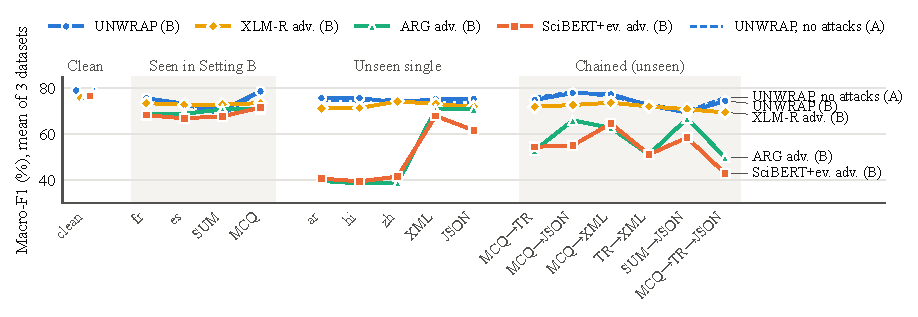
\includegraphics[width=\textwidth]{figures/fig_per_attack.pdf}
\caption{Macro-F1 per attack, averaged over the three datasets, grouped into the attack families seen in Setting~B training, unseen single attacks and unseen chained attacks. Solid lines: all detectors trained on the same transformed claims (Setting~B; \method{} with one seed, the others averaged over three). Dashed line: \method{} trained on clean claims only (Setting~A). Adversarial training of SciBERT with evidence and ARG helps on the seen families and on XML/JSON, which keep much of the claim's wording, but not on unseen languages or chains; \method{} is almost equally robust with and without transformed training claims. Per-dataset numbers are in Table~\ref{tab:seen_unseen} and Tables~\ref{tab:per_pubhealth}--\ref{tab:per_finfact} in the appendix.}
\label{fig:per_attack}
\end{figure*}

\subsection{Seen and unseen attack families}

Setting~B trains on four attack families only: French and Spanish translation, summarisation and multiple-choice questions. Figure~\ref{fig:per_attack} and Table~\ref{tab:seen_unseen} in the appendix separate the test attacks into these seen families, unseen single attacks and the six chains. Adversarial training of SciBERT with evidence and of ARG fails to transfer: on PUBHEALTH they reach 69.6 and 70.5 on seen families but 42.1 and 44.2 on unseen single attacks, and the pattern holds on the other datasets. Trained on the same transformed claims, \method{} beats both by 12.7 to 34.2 points on unseen single attacks and by 9.2 to 28.1 points on chains on every dataset ($p\le0.004$), but by only 0.5 to 7.7 points on the seen families (not significantly on CLIMATE-FEVER). Adversarially trained XLM-R barely varies across groups, plausibly thanks to multilingual pretraining; \method{} is equally flat and better than it in every group on PUBHEALTH and Fin-Fact (+4.1 to +6.5 points, $p\le0.004$), with no significant difference on CLIMATE-FEVER. \method{} trained on clean claims only follows almost the same curve (dashed), so its robustness to unseen attacks does not depend on seeing transformed claims.

\subsection{Ablations}
\label{sec:ablation}

Table~\ref{tab:ablation} changes one component at a time, at the first seed. Canonicalisation is the only retrieval-side component with a significant effect under attack: without it, attacked macro-F1 falls by 9.1 points on CLIMATE-FEVER and 4.6 on Fin-Fact ($p<0.001$) and is unchanged on PUBHEALTH, whereas clean macro-F1 rises by 2.7 to 7.1 points (significantly on PUBHEALTH and CLIMATE-FEVER), presumably because rewriting a claim that is already plain can only lose information. A generic claim-normalisation prompt \citep{sundriyal2023claimnorm} changes no result significantly, so the benefit comes from verifying a normalised claim rather than from our particular instruction. Replacing canonicalisation with the \air{} encoder recovers part of the loss on CLIMATE-FEVER and Fin-Fact and helps slightly on PUBHEALTH (+1.4 points, $p=0.012$). Removing sparse retrieval or the reranker, replacing BGE-M3 by mE5 \citep{wang2024me5}, or adding the \air{} encoder to canonicalisation changes attacked macro-F1 by at most 2.1 points, never significantly. Verifier training matters most: without it, macro-F1 is 6.1 to 12.0 points lower on clean claims and 7.0 to 10.8 points lower under attack ($p<0.001$).

\subsection{Further analyses}

Appendix~\ref{sec:appendix_analyses} reports three further analyses. In front of untrained or zero-shot detectors, \method{}'s canonicaliser significantly raises attacked macro-F1 in 13 of 15 detector--dataset pairs but costs clean accuracy. Of two adaptive attacks on the canonicaliser, an injected instruction to report a decoy claim costs \method{} 2.9 to 5.1 points, whereas three true decoy claims around the content cost 8.8 to 14.0 points, the clearest weakness we found. A guided-instruction contamination test \citep{golchin2024timetravel} finds no memorisation of the test claims by Llama-3.1-8B, the model behind our canonicaliser and verifier, and clear contamination for Claude Opus~5.5 only on CLIMATE-FEVER, where it completes 21 of 97 test claims verbatim.

\section{Conclusion}

Format-shifting attacks preserve the meaning of a false claim and change only how it is presented, yet they reduce many published misinformation detectors and zero-shot LLMs to near or below chance level on three benchmarks. Adversarial training on transformed claims repairs the attack families it covers but, for most detectors, not new languages, formats or chains. \method{} instead verifies the claim: it keeps its clean accuracy, loses about five points under fifteen attacks and, compared under the same training conditions, is significantly more robust than every baseline in 32 of 33 comparisons. Its clearest weakness is an adaptive attacker who surrounds the claim with decoys, which future work could address by verifying every claim a text asserts rather than the most central few.

\section*{Limitations}

\method{} relies on an archive of verified claims, so it can only help with claims that are related to previously fact-checked ones; truly novel claims fall back on the evidence the verifier receives. The benchmark claims are in English, so the translation attacks go from English to other languages and are read back by an English-centric pipeline; claims originally written in other languages may behave differently. Two of our three splits are our own, because CLIMATE-FEVER has no official split and Fin-Fact's test labels are not public, so our numbers are not directly comparable with papers that use other splits. All test attacks come from one attacker model and preservation was judged by one judge model; although both belong to families different from our detector, other attackers may produce harder transformations. We study binary true/false labels and drop mixed or unproven verdicts. For cost reasons, Claude Opus~5.5 was evaluated on 100 claims per dataset only, which leaves some of its comparisons without significance, and its contamination check suggests that its clean score on CLIMATE-FEVER is optimistic. Our contamination check extracts a guess from answers that begin with a hedge, and this extraction is heuristic. Finally, our adaptive attacks are two simple strategies; attackers with more knowledge or query access could design stronger ones, and the Setting~B variant of \method{} and the ablations were run with a single seed.

\section*{Ethics Statement}

The attacks we study use only routine LLM operations such as translation, summarisation and formatting, which are already available to anyone, and we describe them so that detectors can be evaluated and hardened against them. We release attacked versions of public benchmarks only, generated from claims that have already been publicly fact-checked, together with their original verdicts, so the release does not add new misinformation to circulation. Automated detectors make errors that fall unevenly on different topics and communities; we see them as tools that prioritise content for human fact-checkers rather than as replacements for them. The decoy attack in Section~\ref{sec:analysis} shows a weakness of our own method, which we report so that deployments can account for it.

\bibliography{references}

\appendix
\section{Data, attack examples and preservation}
\label{sec:appendix_attacks}

\begin{table}[t]\centering\small\setlength{\tabcolsep}{4pt}
\begin{tabular}{lrrrr}
\toprule
Dataset & Train & Dev & Test & False (\%) \\
\midrule
PUBHEALTH & 8,077 & 1,009 & 985 & 37 \\
CLIMATE-FEVER & 544 & 90 & 272 & 28 \\
Fin-Fact & 1,929 & 275 & 551 & 54 \\
\bottomrule
\end{tabular}
\caption{Binary true/false subsets used in this work (claims per split, and share of false claims). PUBHEALTH uses its official split; CLIMATE-FEVER and Fin-Fact are split by us (stratified, seed 13), and we release the split identifiers.}
\label{tab:data}
\end{table}


Table~\ref{tab:data} gives the size of each split. Tables~\ref{tab:example_single} and~\ref{tab:example_chain} show one false PUBHEALTH test claim under every attack, exactly as given to the detectors. Table~\ref{tab:preservation} gives the share of attacked texts that the judge found to preserve the claim; its prompt is in Appendix~\ref{sec:appendix_prompts}.

\begin{table*}[t]\centering\footnotesize
\begin{tabular}{@{}p{0.13\textwidth}p{0.84\textwidth}@{}}
\toprule
Attack & Text given to the detector \\
\midrule
Clean & Eating more fish could prevent Parkinson's disease \\ \midrule
Translate fr & Translate from French to English: \newline \emph{[French text]} \\
Translate es & Translate from Spanish to English: \newline \emph{[Spanish text]} \\
Translate ar & Translate from Arabic to English: \newline \emph{[Arabic text]} \\
Translate hi & Translate from Hindi to English: \newline \emph{[Hindi text]} \\
Translate zh & Translate from Chinese to English: \newline \emph{[Chinese text]} \\
Summarise & Summarize the following text in one block in five lines: The headline "Eating more fish could prevent Parkinson's disease" suggests a potential dietary approach to mitigating the risk of developing Parkinson's disease, a progressive disorder of the nervous system that affects movement. This headline encapsulates a growing body of research that explores the connection between [...] \\
MCQ & Answer the following question: Why might eating more fish be beneficial according to recent studies? A) It increases muscle mass. B) It prevents Parkinson's disease. C) It improves vision. D) It enhances cognitive abilities in the elderly. \\
XML & Parse the following XML document and rewrite its content as plain English text: \textless{}document\textgreater{} \textless{}headline\textgreater{} Consuming a higher quantity of fish in one's diet might help in reducing the risk of developing Parkinson's disease. \textless{}/headline\textgreater{} \textless{}description\textgreater{} Parkinson's disease is a progressive disorder of the nervous system that affects movement, often leading to symptoms such as [...] \\
JSON & Parse the following JSON object and rewrite its content as plain English text: \{ "headline": "Consuming a higher quantity of fish in one's diet might help in reducing the risk of developing Parkinson's disease", "parkinsons\_disease\_description": "Parkinson's disease is a progressive disorder of the nervous system that affects movement, often leading to symptoms such as tremors, [...] \\
\bottomrule
\end{tabular}
\caption{One false PUBHEALTH test claim under the single attacks, as given to the detectors (the attack text and its task wrapper). Long texts are cut after 55 words ([...]); texts in other languages are described in brackets rather than shown. The judge found that every attacked version preserves the claim.}
\label{tab:example_single}
\end{table*}

\begin{table*}[t]\centering\footnotesize
\begin{tabular}{@{}p{0.13\textwidth}p{0.84\textwidth}@{}}
\toprule
Attack & Text given to the detector \\
\midrule
MCQ$\to$TR & Translate the following question from Spanish to English and answer it: \newline \emph{[multiple-choice question in Spanish]} \\
MCQ$\to$JSON & The following JSON object contains a multiple-choice question. Parse it and answer the question: \{ "question": "Why might eating more fish be beneficial according to recent studies?", "options": \{ "A": "It increases muscle mass.", "B": "It prevents Parkinson's disease.", "C": "It improves vision.", "D": "It enhances cognitive abilities in the elderly." \} \} \\
MCQ$\to$XML & The following XML document contains a multiple-choice question. Parse it and answer the question: \textless{}document\textgreater{} \textless{}question\textgreater{}Why might eating more fish be beneficial according to recent studies?\textless{}/question\textgreater{} \textless{}options\textgreater{} \textless{}option id="A"\textgreater{}It increases muscle mass.\textless{}/option\textgreater{} \textless{}option id="B"\textgreater{}It prevents Parkinson's disease.\textless{}/option\textgreater{} \textless{}option id="C"\textgreater{}It improves vision.\textless{}/option\textgreater{} \textless{}option id="D"\textgreater{}It enhances cognitive abilities in the elderly.\textless{}/option\textgreater{} \textless{}/options\textgreater{} \textless{}/document\textgreater{} \\
TR$\to$XML & Parse the following XML document, whose text is in Spanish, and translate its content to English: \newline \emph{[XML document in Spanish]} \\
Summarise$\to$JSON & Parse the following JSON object and summarize its content in one block in five lines: \{ "headline": "Eating more fish could prevent Parkinson's disease", "summary": "Suggests a potential dietary approach to mitigating the risk of developing Parkinson's disease, a progressive disorder of the nervous system affecting movement.", "details": \{ "disease\_characteristics": "Characterized by the loss of [...] \\
MCQ$\to$TR$\to$JSON & The following JSON object contains a multiple-choice question in Spanish. Parse it, translate the question to English, and answer it: \newline \emph{[JSON object containing a multiple-choice question in Spanish]} \\
\bottomrule
\end{tabular}
\caption{One false PUBHEALTH test claim under the chained attacks, as given to the detectors (the attack text and its task wrapper). Long texts are cut after 55 words ([...]); texts in other languages are described in brackets rather than shown. The judge found that every attacked version preserves the claim. The chained translations of this claim are into Spanish.}
\label{tab:example_chain}
\end{table*}

\begin{table}[t]\centering\small
\begin{adjustbox}{max width=\columnwidth}\begin{tabular}{lccc}
\toprule
Attack & PUBH. & C-FEVER & Fin-Fact \\
\midrule
fr & 91.4 & 89.7 & 89.3 \\
es & 91.0 & 89.3 & 88.6 \\
ar & 91.8 & 89.3 & 89.5 \\
hi & 91.4 & 90.4 & 90.6 \\
zh & 91.3 & 90.4 & 89.1 \\
SUM & 90.6 & 83.8 & 82.8 \\
MCQ & 98.8 & 98.9 & 96.2 \\
XML & 92.0 & 90.8 & 91.1 \\
JSON & 92.0 & 92.3 & 91.5 \\
MCQ$\to$TR & 98.4 & 97.8 & 96.7 \\
MCQ$\to$JSON & 98.8 & 98.9 & 95.8 \\
MCQ$\to$XML & 98.7 & 97.4 & 92.9 \\
TR$\to$XML & 92.0 & 89.3 & 89.3 \\
SUM$\to$JSON & 92.5 & 84.6 & 86.4 \\
MCQ$\to$TR$\to$JSON & 98.1 & 97.4 & 94.6 \\
\midrule
All & 93.9 & 92.0 & 90.9 \\
\quad false claims & 85.9 & 78.0 & 86.8 \\
\quad true claims & 99.1 & 97.5 & 95.8 \\
\bottomrule
\end{tabular}\end{adjustbox}
\caption{Share (\%) of attacked test texts that the Gemma-3-12B judge found to preserve the original claim.}
\label{tab:preservation}
\end{table}


\section{Further analyses}
\label{sec:appendix_analyses}

\subsection{Canonicalisation as a plug-in defence}

Placing \method{}'s canonicaliser in front of an existing detector significantly raises its attacked macro-F1 in 13 of 15 detector--dataset pairs for detectors trained on clean claims or used zero-shot, by up to 18.7 points (XLM-R on PUBHEALTH), and lowers it once (claim retrieval on Fin-Fact, $-5.4$ points; Table~\ref{tab:plugin}). The gain is paid for on clean claims: zero-shot Llama loses 7.9 to 12.2 points of clean macro-F1, and XLM-R loses 19.0 points on PUBHEALTH, presumably because these detectors were developed or trained on claims as published rather than on their canonical rewrites. For adversarially trained XLM-R, which is already robust, the canonicaliser hurts under attack ($-1.9$ points on PUBHEALTH and $-7.9$ on CLIMATE-FEVER). Canonicalisation is therefore most useful together with a verifier that is trained on canonical claims, as in \method{}.

\subsection{Adaptive attacks}

We evaluate two adaptive attacks by an attacker who knows our pipeline. The \emph{injection} attack inserts, before and after the content, a note addressed to automated claim-extraction systems, stating that the text's only claim is a decoy, namely a true claim from the training split. The \emph{decoy} attack surrounds the content with three true training claims to push the real claim out of the canonicaliser's output. Both are applied on top of the MCQ$\rightarrow$JSON and summarisation attacks.

An attacker who knows that \method{} canonicalises its input can target that step (Table~\ref{tab:adaptive}). An injected note that tells claim extractors to report a decoy claim lowers \method{}'s macro-F1 by 2.9 to 5.1 points relative to the same attacks without it, a loss similar to that of adversarially trained XLM-R (4.9 to 6.9 points), which has no extraction step. Surrounding the content with three true decoy claims is more effective and lowers \method{} by 8.8 to 14.0 points, more than XLM-R on PUBHEALTH and Fin-Fact; the Setting~B variant of \method{} is affected more than the Setting~A variant on all three datasets, by 11.7 to 17.8 points. Decoys plausibly exploit the canonicaliser's limit of three claims and its ordering by centrality, and they are the clearest weakness we found. We note that decoy texts also preserve the original claim less often according to the judge, as low as 48.5\% for MCQ$\rightarrow$JSON on CLIMATE-FEVER, so the attacker pays for the attack with a less effective message.

\subsection{Test-set contamination}
\label{sec:contamination}

LLM-based detectors may have seen the benchmark claims, and their verdicts, during pretraining. We test Llama-3.1-8B-Instruct, the canonicaliser and verifier of \method{}, and Claude Opus~5.5 with the guided instruction method of \citet{golchin2024timetravel}: given the first part of a test claim, the model completes it once with an instruction that names the dataset and split (guided) and once without (general), and contamination is indicated when the guided completions are significantly closer to the true claim. In the original instruction format, Llama refused 95 to 100\% of the guided prompts, so we pre-fill the answer with the first part of the claim, which reduces refusals to at most 1.2\%. Table~\ref{tab:contamination} shows that the completions are far from the true claims (ROUGE-L \citep{lin2004rouge} of 0.08 to 0.13) and only one of 280 claims is reproduced exactly. Naming the dataset raises ROUGE-L slightly but significantly on PUBHEALTH and CLIMATE-FEVER, by 0.037 and 0.038, which may reflect topic priming as well as exposure, and not on Fin-Fact. Some guided prompts produced no completion; restricting the test to claims with two non-empty completions gives the same conclusions. Since the same model also serves as the zero-shot baseline, which is not robust, exposure to the claims does not explain the results.

For Claude Opus~5.5 the picture depends on the dataset. Claude usually prefaces its guided answer with a statement that it cannot recall the exact wording (52 to 79\% of guided answers) and then gives a guess, which we extract and score. On CLIMATE-FEVER, its guided completions reproduce the second piece of 21 of 97 claims exactly, 13 of them with eight or more words, against a single exact completion with the general instruction; a verbatim continuation of that length is very unlikely to be guessed, so we conclude that Claude has seen many CLIMATE-FEVER claims, or the widely republished sources they were taken from. On PUBHEALTH and Fin-Fact, naming the dataset hardly changes exact reproduction (5 vs.\ 2 and 5 vs.\ 5 exact completions, mostly short and predictable endings), and the one long Fin-Fact match is a well-known quotation that Claude also completes without the dataset name; guided ROUGE-L is significantly higher on both datasets ($p<0.001$), but, as for Llama, this gain may reflect topic priming. We therefore find clear evidence of contamination only for CLIMATE-FEVER, where Claude's clean score may overstate what it would achieve on unseen claims. This makes its loss under attack there more telling: claims the model has probably seen are still missed once their format is shifted.

\section{Additional results}
\label{sec:appendix_results}

\begin{table*}[t]\centering\small\setlength{\tabcolsep}{5pt}
\begin{adjustbox}{max width=\textwidth}\begin{tabular}{lccccccccc}
\toprule
 & \multicolumn{3}{c}{PUBHEALTH} & \multicolumn{3}{c}{CLIMATE-FEVER} & \multicolumn{3}{c}{Fin-Fact} \\
\cmidrule(lr){2-4} \cmidrule(lr){5-7} \cmidrule(lr){8-10}
Detector & Clean & Att. & $\Delta$ & Clean & Att. & $\Delta$ & Clean & Att. & $\Delta$ \\
\midrule
Claude Opus 5.5 zero-shot \citep{anthropic2026opus55} & 85.8 & 68.9 & $-16.9$ & 70.5 & 55.2 & $-15.4$ & 49.5 & 59.8 & $+10.3$ \\
Llama-3.1-8B zero-shot \citep{grattafiori2024llama3} & 81.1 & 48.0$^{*}$ & $-33.1$ & 69.9 & 43.7$^{*}$ & $-26.2$ & 57.5 & 38.8$^{*}$ & $-18.7$ \\
Claim retrieval + LLM \citep{pikuliak2023multiclaim} & 74.1$^{*}$ & 62.3 & $-11.7$ & 74.0 & 48.9 & $-25.1$ & 68.0$^{*}$ & 64.4 & $-3.6$ \\
XLM-R, adv.\ training \citep{conneau2020xlmr} (B) & 79.4 & 71.1 & $-8.4$ & 67.8 & 69.3$^{*}$ & $+1.5$ & 75.5$^{*}$ & 71.0$^{*}$ & $-4.5$ \\
\method{} (ours, A) & 87.1 & 76.7 & $-10.4$ & 77.7 & 68.6$^{*}$ & $-9.0$ & 78.3$^{*}$ & 73.1$^{*}$ & $-5.2$ \\
\method{} + \air{} + aug.\ (ours, B) & 79.2 & 72.7 & $-6.5$ & 72.4 & 64.2 & $-8.2$ & 76.7$^{*}$ & 74.6$^{*}$ & $-2.1$ \\
\bottomrule
\end{tabular}\end{adjustbox}
\caption{Claude Opus 5.5 compared with selected detectors on the same stratified subsample of 100 test claims per dataset, clean and under the fifteen attacks (macro-F1, \%). Claude was run on this subsample only, for cost reasons, so all detectors here are rescored on the same 100 claims; their numbers therefore differ slightly from Table~\ref{tab:main}, which uses the full test sets. $^{*}$: significantly different from Claude (paired bootstrap, $p<0.05$). Answers that are neither yes nor no (1 of 4800) count as not flagged. \method{} + \air{} + aug.: the Setting~B variant of \method{}, with the attack-invariant retriever (\air{}) and a verifier also trained on the transformed (augmented) training claims.}
\label{tab:claude}
\end{table*}

\begin{table*}[t]\centering\small\setlength{\tabcolsep}{5pt}
\begin{adjustbox}{max width=\textwidth}\begin{tabular}{lccccccccc}
\toprule
 & \multicolumn{3}{c}{PUBHEALTH} & \multicolumn{3}{c}{CLIMATE-FEVER} & \multicolumn{3}{c}{Fin-Fact} \\
\cmidrule(lr){2-4} \cmidrule(lr){5-7} \cmidrule(lr){8-10}
Detector & Seen & Unseen & Chains & Seen & Unseen & Chains & Seen & Unseen & Chains \\
\midrule
\multicolumn{10}{l}{\emph{Setting A}} \\
SciBERT + evidence & 42.3 & 29.4 & 29.8 & 47.1 & 38.7 & 47.2 & 56.7 & 48.0 & 49.8 \\
ARG & 32.7 & 30.7 & 29.2 & 35.1 & 27.2 & 26.0 & 52.3 & 39.2 & 45.9 \\
XLM-R & 42.1 & 38.3 & 31.3 & 45.2 & 42.8 & 44.7 & 52.4 & 51.6 & 54.2 \\
\method{} & 75.7 & 75.8 & 78.2 & 69.1 & 73.1 & 71.4 & 76.0 & 74.3 & 75.3 \\
\midrule
\multicolumn{10}{l}{\emph{Setting B}} \\
SciBERT + evidence & 69.6 & 42.1 & 49.2 & 62.7 & 51.5 & 55.2 & 73.7 & 57.3 & 59.2 \\
ARG & 70.5 & 44.2 & 52.1 & 67.8 & 58.6 & 59.3 & 71.2 & 52.5 & 63.4 \\
XLM-R & 72.4 & 71.1 & 70.8 & 72.8 & 72.6 & 71.7 & 74.4 & 73.5 & 72.9 \\
\method{} + \air{} + aug. & 76.5 & 76.4 & 77.3 & 68.3 & 71.3 & 68.5 & 78.8 & 77.9 & 77.6 \\
\bottomrule
\end{tabular}\end{adjustbox}
\caption{Macro-F1 (\%) by attack group. Setting~B adds transformed training claims of four attack families only. Seen: test attacks of these families (French and Spanish translation, summarisation, MCQ); the training copies were produced by a different model and instructions than the test attacks, so the type is seen but not the texts. Unseen: single attacks of families absent from training (Arabic, Hindi and Chinese translation, XML, JSON). Chains: the six chained attacks, never seen as such. Setting~A models saw no attacks at all; their rows use the same split for comparison.}
\label{tab:seen_unseen}
\end{table*}

\begin{table*}[t]\centering\small\setlength{\tabcolsep}{2.8pt}
\begin{adjustbox}{max width=\textwidth}\begin{tabular}{lcccccccccccc}
\toprule
 & \multicolumn{4}{c}{PUBHEALTH} & \multicolumn{4}{c}{CLIMATE-FEVER} & \multicolumn{4}{c}{Fin-Fact} \\
\cmidrule(lr){2-5} \cmidrule(lr){6-9} \cmidrule(lr){10-13}
 & \multicolumn{2}{c}{Clean} & \multicolumn{2}{c}{Att.} & \multicolumn{2}{c}{Clean} & \multicolumn{2}{c}{Att.} & \multicolumn{2}{c}{Clean} & \multicolumn{2}{c}{Att.} \\
Detector & w/o & with & w/o & with & w/o & with & w/o & with & w/o & with & w/o & with \\
\midrule
XLM-R \citep{conneau2020xlmr} & 79.9 & 60.9$^{*}$ & 36.5 & 55.2$^{*}$ & 53.5 & 54.0 & 44.2 & 48.0$^{*}$ & 71.4 & 63.7$^{*}$ & 52.8 & 62.3$^{*}$ \\
XLM-R, adv.\ training \citep{conneau2020xlmr} & 79.4 & 71.2$^{*}$ & 71.3 & 69.5$^{*}$ & 72.0 & 65.2 & 72.3 & 64.4$^{*}$ & 76.4 & 73.6 & 73.5 & 73.5 \\
Llama-3.1-8B zero-shot \citep{grattafiori2024llama3} & 77.6 & 68.2$^{*}$ & 47.5 & 58.4$^{*}$ & 73.5 & 61.3$^{*}$ & 43.1 & 59.3$^{*}$ & 58.1 & 50.2$^{*}$ & 39.5 & 48.2$^{*}$ \\
Qwen2.5-7B zero-shot \citep{qwen2024qwen25} & 60.6 & 62.6 & 49.0 & 59.1$^{*}$ & 42.2 & 52.9$^{*}$ & 48.7 & 55.5$^{*}$ & 44.2 & 48.6 & 47.2 & 49.7$^{*}$ \\
Claim retrieval + LLM \citep{pikuliak2023multiclaim} & 77.7 & 72.1$^{*}$ & 60.3 & 65.5$^{*}$ & 72.7 & 76.1 & 48.8 & 61.5$^{*}$ & 75.1 & 63.9$^{*}$ & 67.6 & 62.3$^{*}$ \\
MiniCheck \citep{tang2024minicheck} & 57.0 & 56.7 & 43.2 & 51.5$^{*}$ & 67.7 & 58.0$^{*}$ & 46.2 & 48.8 & 49.7 & 53.1 & 37.1 & 48.3$^{*}$ \\
\bottomrule
\end{tabular}\end{adjustbox}
\caption{Macro-F1 (\%) of existing detectors without (w/o) and with \method{}'s canonicaliser in front of them, on clean claims and averaged over the fifteen attacks. $^{*}$: significant change (paired bootstrap, $p<0.05$).}
\label{tab:plugin}
\end{table*}

\begin{table*}[t]\centering\small\setlength{\tabcolsep}{5pt}
\begin{adjustbox}{max width=\textwidth}\begin{tabular}{lccccccccc}
\toprule
 & \multicolumn{3}{c}{PUBHEALTH} & \multicolumn{3}{c}{CLIMATE-FEVER} & \multicolumn{3}{c}{Fin-Fact} \\
\cmidrule(lr){2-4} \cmidrule(lr){5-7} \cmidrule(lr){8-10}
Detector & Base & Inj. & Decoy & Base & Inj. & Decoy & Base & Inj. & Decoy \\
\midrule
Claim retrieval + LLM \citep{pikuliak2023multiclaim} & 63.3 & 61.3 & 56.0 & 45.9 & 47.8 & 45.2 & 65.8 & 64.0 & 57.6 \\
XLM-R, adv.\ training \citep{conneau2020xlmr} & 72.1 & 66.4 & 66.8 & 71.8 & 66.9 & 58.6 & 74.6 & 67.7 & 67.4 \\
\method{} (ours) & 75.9 & 72.8 & 67.2 & 68.1 & 65.3 & 56.8 & 76.6 & 71.4 & 62.6 \\
\method{} + \air{} + aug. (ours) & 77.3 & 70.9 & 65.5 & 66.2 & 54.4 & 48.4 & 79.3 & 70.4 & 62.3 \\
\bottomrule
\end{tabular}\end{adjustbox}
\caption{Adaptive attacks. Macro-F1 (\%) averaged over the summarisation and MCQ$\rightarrow$JSON attacks, without (Base) and with an injected instruction to the claim extractor (Inj.) or three true decoy claims around the content (Decoy). \method{} + \air{} + aug.: the Setting~B variant of \method{}, with the attack-invariant retriever (\air{}) and a verifier also trained on the transformed (augmented) training claims.}
\label{tab:adaptive}
\end{table*}

\begin{table*}[t]\centering\small\setlength{\tabcolsep}{5pt}
\begin{adjustbox}{max width=\textwidth}\begin{tabular}{lcccccc}
\toprule
 & \multicolumn{3}{c}{Llama-3.1-8B-Instruct (answer pre-filled)} & \multicolumn{3}{c}{Claude Opus 5.5 (instruction format)} \\
\cmidrule(lr){2-4} \cmidrule(lr){5-7}
 & PUBH. & C-FEVER & Fin-Fact & PUBH. & C-FEVER & Fin-Fact \\
\midrule
Claims tested & 99 & 97 & 84 & 99 & 97 & 84 \\
ROUGE-L, guided & 0.114 & 0.133 & 0.080 & 0.277 & 0.418 & 0.293 \\
ROUGE-L, general & 0.078 & 0.095 & 0.089 & 0.149 & 0.167 & 0.223 \\
One-sided $p$ (guided $>$ general) & $<$0.0001 & 0.0006 & 0.791 & $<$0.0001 & $<$0.0001 & 0.0004 \\
\quad non-empty pairs only & $<$0.0001 & $<$0.0001 & 0.158 & -- & -- & -- \\
Exact, guided & 1 & 0 & 0 & 5 & 21 & 5 \\
Near-exact, guided & 0 & 0 & 1 & 4 & 6 & 6 \\
Exact, general & 0 & 0 & 0 & 2 & 1 & 5 \\
Guided answers refused or hedged$^{a}$ & 100\% & 100\% & 95\% & 79\% & 52\% & 73\% \\
\bottomrule
\end{tabular}\end{adjustbox}
\caption{Guided instruction test for test-set contamination \citep{golchin2024timetravel}: the model completes the first piece of a test claim once with an instruction naming the dataset and split (guided) and once without (general). ROUGE-L is computed on the generated second piece; $p$ tests guided $>$ general (10,000 bootstrap resamples); near-exact means ROUGE-L $\geq 0.75$. $^{a}$For Llama, in the instruction format, which it refused almost entirely, so its test uses a pre-filled answer; some of its guided completions were then empty (scored 0), and the test without them is also given. Claude usually hedges before giving a guess, which is extracted and scored.}
\label{tab:contamination}
\end{table*}

\begin{table*}[t]\centering\small\setlength{\tabcolsep}{4.5pt}
\begin{adjustbox}{max width=\textwidth}\begin{tabular}{lcccccccccc}
\toprule
\multicolumn{11}{l}{\emph{Clean and single attacks}} \\
Detector & Clean & fr & es & ar & hi & zh & SUM & MCQ & XML & JSON \\
\midrule
ProgramFC & 54.8 & 45.9 & 44.2 & 46.8 & 47.6 & 50.4 & 36.5 & 54.4 & 40.0 & 39.2 \\
MiniCheck & 57.0 & 46.0 & 44.5 & 39.5 & 39.5 & 42.0 & 43.0 & 46.6 & 41.1 & 41.9 \\
Claim retrieval + LLM & 77.7 & 58.4 & 59.5 & 58.4 & 58.8 & 60.5 & 62.6 & 64.8 & 56.3 & 60.3 \\
Llama-3.1-8B zero-shot & 77.6 & 43.9 & 40.0 & 43.7 & 47.0 & 40.8 & 51.3 & 45.1 & 42.6 & 42.1 \\
Qwen2.5-7B zero-shot & 60.6 & 49.8 & 46.6 & 53.3 & 56.4 & 51.6 & 39.4 & 47.3 & 44.5 & 50.4 \\
\method{}, no training & 70.9 & 65.4 & 65.4 & 65.2 & 69.4 & 68.1 & 59.5 & 68.9 & 67.0 & 65.4 \\
SciBERT + evidence & 79.2 & 46.9 & 30.2 & 25.7 & 29.5 & 25.8 & 49.8 & 42.3 & 37.8 & 28.1 \\
ARG & 79.8 & 26.8 & 25.6 & 26.0 & 25.8 & 25.5 & 46.0 & 32.2 & 43.3 & 32.9 \\
XLM-R & 79.9 & 43.1 & 48.1 & 37.6 & 45.3 & 41.6 & 40.8 & 36.5 & 34.9 & 31.8 \\
\method{} & 82.0 & 76.1 & 75.6 & 75.4 & 75.9 & 74.5 & 70.5 & 80.6 & 76.6 & 76.5 \\
\cmidrule(lr){1-11}
SciBERT + evidence, adv. & 79.4 & 68.0 & 68.7 & 26.6 & 27.3 & 27.8 & 70.2 & 71.2 & 68.8 & 60.2 \\
ARG, adv. & 79.7 & 68.2 & 68.7 & 30.7 & 26.1 & 25.5 & 72.6 & 72.6 & 71.7 & 67.1 \\
XLM-R, adv. & 79.4 & 71.2 & 71.4 & 69.1 & 70.2 & 72.5 & 73.2 & 73.7 & 72.7 & 71.2 \\
\method{} + \air{} + aug. & 79.4 & 76.3 & 75.8 & 75.6 & 76.8 & 75.8 & 73.9 & 79.8 & 77.6 & 76.0 \\
\midrule
\multicolumn{11}{l}{\emph{Chained attacks}} \\
Detector & C1 & C2 & C3 & C4 & C5 & C6 &  &  &  &  \\
\midrule
ProgramFC & 49.0 & 49.2 & 43.7 & 33.7 & 34.5 & 43.9 &  &  &  &  \\
MiniCheck & 44.7 & 44.8 & 50.5 & 40.4 & 40.1 & 43.7 &  &  &  &  \\
Claim retrieval + LLM & 65.7 & 64.0 & 66.5 & 51.0 & 55.1 & 62.5 &  &  &  &  \\
Llama-3.1-8B zero-shot & 63.2 & 62.1 & 61.4 & 41.4 & 42.3 & 46.2 &  &  &  &  \\
Qwen2.5-7B zero-shot & 57.5 & 51.7 & 44.1 & 49.4 & 51.9 & 41.0 &  &  &  &  \\
\method{}, no training & 65.0 & 68.2 & 70.9 & 65.4 & 63.7 & 66.6 &  &  &  &  \\
SciBERT + evidence & 29.2 & 28.1 & 33.3 & 27.8 & 32.4 & 28.0 &  &  &  &  \\
ARG & 28.3 & 28.0 & 29.2 & 27.7 & 33.5 & 28.2 &  &  &  &  \\
XLM-R & 31.4 & 28.5 & 29.7 & 36.6 & 32.8 & 28.9 &  &  &  &  \\
\method{} & 78.9 & 81.4 & 80.2 & 75.5 & 74.2 & 79.0 &  &  &  &  \\
\cmidrule(lr){1-11}
SciBERT + evidence, adv. & 45.7 & 48.4 & 62.2 & 45.3 & 59.6 & 34.0 &  &  &  &  \\
ARG, adv. & 46.1 & 58.6 & 54.1 & 48.6 & 67.3 & 38.2 &  &  &  &  \\
XLM-R, adv. & 70.9 & 71.0 & 73.7 & 70.8 & 72.7 & 65.6 &  &  &  &  \\
\method{} + \air{} + aug. & 76.5 & 80.7 & 79.5 & 75.1 & 74.9 & 77.0 &  &  &  &  \\
\bottomrule
\end{tabular}\end{adjustbox}
\caption{Macro-F1 (\%) per attack on PUBHEALTH. Chained attacks: C1 = MCQ$\to$TR, C2 = MCQ$\to$JSON, C3 = MCQ$\to$XML, C4 = TR$\to$XML, C5 = SUM$\to$JSON, C6 = MCQ$\to$TR$\to$JSON. Rows above the inner rule are trained on clean claims only (Setting~A), rows below also on transformed training claims (Setting~B).}
\label{tab:per_pubhealth}
\end{table*}

\begin{table*}[t]\centering\small\setlength{\tabcolsep}{4.5pt}
\begin{adjustbox}{max width=\textwidth}\begin{tabular}{lcccccccccc}
\toprule
\multicolumn{11}{l}{\emph{Clean and single attacks}} \\
Detector & Clean & fr & es & ar & hi & zh & SUM & MCQ & XML & JSON \\
\midrule
ProgramFC \citep{pan2023programfc} & 54.7 & 43.4 & 45.1 & 47.4 & 40.5 & 37.2 & 27.6 & 53.1 & 44.5 & 43.0 \\
MiniCheck \citep{tang2024minicheck} & 67.7 & 45.2 & 44.5 & 43.8 & 43.7 & 43.4 & 44.7 & 48.0 & 45.3 & 46.6 \\
Claim retrieval + LLM \citep{pikuliak2023multiclaim} & 72.7 & 47.6 & 45.8 & 45.8 & 47.4 & 45.4 & 44.5 & 56.2 & 50.4 & 51.9 \\
Llama-3.1-8B zero-shot \citep{grattafiori2024llama3} & 73.5 & 43.8 & 43.9 & 43.9 & 43.6 & 43.6 & 44.7 & 38.6 & 43.5 & 43.2 \\
Qwen2.5-7B zero-shot \citep{qwen2024qwen25} & 42.2 & 52.4 & 57.5 & 52.0 & 58.9 & 62.7 & 27.5 & 30.0 & 55.4 & 66.7 \\
\method{}, no training (ours) & 69.4 & 66.9 & 64.9 & 65.3 & 64.4 & 69.1 & 55.1 & 66.7 & 66.1 & 62.9 \\
SciBERT + evidence \citep{kotonya2020pubhealth} & 69.1 & 42.5 & 39.6 & 20.7 & 39.3 & 33.0 & 52.0 & 54.2 & 51.8 & 48.7 \\
ARG \citep{hu2024arg} & 49.3 & 18.1 & 17.9 & 17.9 & 18.3 & 18.5 & 51.0 & 53.3 & 39.8 & 41.5 \\
XLM-R \citep{conneau2020xlmr} & 53.5 & 44.8 & 44.5 & 39.0 & 43.6 & 45.2 & 44.7 & 46.8 & 43.3 & 43.1 \\
\method{} (ours) & 77.0 & 72.2 & 68.7 & 74.5 & 72.8 & 76.0 & 58.9 & 76.6 & 70.3 & 72.1 \\
\cmidrule(lr){1-11}
SciBERT + evidence, adv. \citep{kotonya2020pubhealth} & 73.6 & 62.8 & 59.9 & 48.5 & 44.2 & 40.8 & 59.0 & 69.1 & 63.8 & 60.3 \\
ARG, adv. \citep{hu2024arg} & 73.6 & 69.9 & 67.5 & 54.9 & 46.6 & 47.4 & 66.8 & 67.0 & 69.6 & 74.6 \\
XLM-R, adv. \citep{conneau2020xlmr} & 72.0 & 76.0 & 73.0 & 71.6 & 69.7 & 76.4 & 71.0 & 71.4 & 73.6 & 71.7 \\
\method{} + \air{} + aug. (ours) & 77.1 & 71.2 & 67.5 & 73.1 & 71.9 & 68.0 & 60.1 & 74.5 & 71.4 & 72.1 \\
\midrule
\multicolumn{11}{l}{\emph{Chained attacks}} \\
Detector & C1 & C2 & C3 & C4 & C5 & C6 &  &  &  &  \\
\midrule
ProgramFC \citep{pan2023programfc} & 55.1 & 48.7 & 44.0 & 22.1 & 29.7 & 37.5 &  &  &  &  \\
MiniCheck \citep{tang2024minicheck} & 49.6 & 56.2 & 48.6 & 43.9 & 44.7 & 45.0 &  &  &  &  \\
Claim retrieval + LLM \citep{pikuliak2023multiclaim} & 61.6 & 47.3 & 46.6 & 45.8 & 47.0 & 48.9 &  &  &  &  \\
Llama-3.1-8B zero-shot \citep{grattafiori2024llama3} & 43.0 & 42.0 & 42.5 & 43.9 & 44.7 & 42.0 &  &  &  &  \\
Qwen2.5-7B zero-shot \citep{qwen2024qwen25} & 42.6 & 34.9 & 48.6 & 53.5 & 63.3 & 24.5 &  &  &  &  \\
\method{}, no training (ours) & 64.3 & 65.9 & 62.1 & 65.5 & 59.3 & 62.5 &  &  &  &  \\
SciBERT + evidence \citep{kotonya2020pubhealth} & 42.7 & 51.1 & 53.5 & 39.2 & 53.5 & 43.0 &  &  &  &  \\
ARG \citep{hu2024arg} & 21.5 & 28.0 & 29.2 & 17.9 & 38.0 & 21.4 &  &  &  &  \\
XLM-R \citep{conneau2020xlmr} & 46.9 & 42.2 & 42.3 & 45.9 & 44.7 & 45.9 &  &  &  &  \\
\method{} (ours) & 72.4 & 77.4 & 72.1 & 70.4 & 63.2 & 73.0 &  &  &  &  \\
\cmidrule(lr){1-11}
SciBERT + evidence, adv. \citep{kotonya2020pubhealth} & 58.3 & 58.1 & 65.1 & 50.5 & 53.5 & 45.7 &  &  &  &  \\
ARG, adv. \citep{hu2024arg} & 55.9 & 67.3 & 64.7 & 47.8 & 64.0 & 56.2 &  &  &  &  \\
XLM-R, adv. \citep{conneau2020xlmr} & 73.0 & 72.6 & 72.5 & 72.7 & 67.0 & 72.6 &  &  &  &  \\
\method{} + \air{} + aug. (ours) & 71.6 & 72.4 & 72.6 & 65.9 & 58.9 & 69.8 &  &  &  &  \\
\bottomrule
\end{tabular}\end{adjustbox}
\caption{Macro-F1 (\%) per attack on CLIMATE-FEVER. Chained attacks: C1 = MCQ$\to$TR, C2 = MCQ$\to$JSON, C3 = MCQ$\to$XML, C4 = TR$\to$XML, C5 = SUM$\to$JSON, C6 = MCQ$\to$TR$\to$JSON. Rows above the inner rule are trained on clean claims only (Setting~A), rows below also on transformed training claims (Setting~B). \method{} + \air{} + aug.: the Setting~B variant of \method{}, with the attack-invariant retriever (\air{}) and a verifier also trained on the transformed (augmented) training claims.}
\label{tab:per_climatefever}
\end{table*}

\begin{table*}[t]\centering\small\setlength{\tabcolsep}{4.5pt}
\begin{adjustbox}{max width=\textwidth}\begin{tabular}{lcccccccccc}
\toprule
\multicolumn{11}{l}{\emph{Clean and single attacks}} \\
Detector & Clean & fr & es & ar & hi & zh & SUM & MCQ & XML & JSON \\
\midrule
ProgramFC \citep{pan2023programfc} & 52.7 & 48.4 & 51.7 & 47.2 & 50.9 & 47.3 & 38.4 & 54.4 & 42.2 & 41.7 \\
MiniCheck \citep{tang2024minicheck} & 49.7 & 35.6 & 36.3 & 33.0 & 32.8 & 33.4 & 35.0 & 53.7 & 33.6 & 33.4 \\
Claim retrieval + LLM \citep{pikuliak2023multiclaim} & 75.1 & 70.7 & 68.7 & 70.8 & 70.4 & 72.5 & 65.0 & 70.3 & 68.2 & 67.4 \\
Llama-3.1-8B zero-shot \citep{grattafiori2024llama3} & 58.1 & 35.9 & 33.7 & 34.3 & 37.6 & 33.9 & 42.9 & 43.9 & 35.0 & 35.2 \\
Qwen2.5-7B zero-shot \citep{qwen2024qwen25} & 44.2 & 45.5 & 42.5 & 56.3 & 58.5 & 52.3 & 33.5 & 41.2 & 38.9 & 46.5 \\
\method{}, no training (ours) & 66.5 & 67.0 & 67.8 & 69.1 & 67.5 & 68.2 & 69.0 & 72.6 & 66.8 & 66.8 \\
SciBERT + evidence \citep{kotonya2020pubhealth} & 72.8 & 57.6 & 49.7 & 36.1 & 38.9 & 41.0 & 52.7 & 66.7 & 64.1 & 59.8 \\
ARG \citep{hu2024arg} & 72.8 & 62.0 & 38.7 & 32.7 & 32.8 & 33.2 & 43.9 & 64.5 & 48.4 & 48.7 \\
XLM-R \citep{conneau2020xlmr} & 71.4 & 55.9 & 59.7 & 53.1 & 58.6 & 62.7 & 34.3 & 59.7 & 40.5 & 43.1 \\
\method{} (ours) & 79.5 & 74.3 & 74.3 & 75.0 & 74.5 & 74.8 & 76.5 & 79.0 & 73.8 & 73.5 \\
\cmidrule(lr){1-11}
SciBERT + evidence, adv. \citep{kotonya2020pubhealth} & 76.8 & 74.1 & 72.2 & 47.2 & 47.2 & 56.2 & 74.2 & 74.5 & 71.3 & 64.6 \\
ARG, adv. \citep{hu2024arg} & 75.6 & 68.0 & 70.6 & 33.6 & 43.3 & 43.5 & 72.9 & 73.1 & 71.2 & 70.7 \\
XLM-R, adv. \citep{conneau2020xlmr} & 76.4 & 73.4 & 74.1 & 73.1 & 74.2 & 74.0 & 74.5 & 75.5 & 73.2 & 72.8 \\
\method{} + \air{} + aug. (ours) & 80.6 & 79.4 & 76.4 & 78.4 & 78.5 & 77.7 & 77.8 & 81.5 & 76.6 & 78.1 \\
\midrule
\multicolumn{11}{l}{\emph{Chained attacks}} \\
Detector & C1 & C2 & C3 & C4 & C5 & C6 &  &  &  &  \\
\midrule
ProgramFC \citep{pan2023programfc} & 50.4 & 38.9 & 34.5 & 39.3 & 39.2 & 47.4 &  &  &  &  \\
MiniCheck \citep{tang2024minicheck} & 37.1 & 52.1 & 38.2 & 33.2 & 33.5 & 35.4 &  &  &  &  \\
Claim retrieval + LLM \citep{pikuliak2023multiclaim} & 64.8 & 66.7 & 67.0 & 69.0 & 57.2 & 65.8 &  &  &  &  \\
Llama-3.1-8B zero-shot \citep{grattafiori2024llama3} & 53.2 & 51.0 & 49.1 & 34.2 & 35.0 & 37.1 &  &  &  &  \\
Qwen2.5-7B zero-shot \citep{qwen2024qwen25} & 53.9 & 55.4 & 45.7 & 53.8 & 48.2 & 35.4 &  &  &  &  \\
\method{}, no training (ours) & 64.8 & 67.3 & 67.7 & 68.5 & 63.9 & 68.2 &  &  &  &  \\
SciBERT + evidence \citep{kotonya2020pubhealth} & 40.1 & 58.2 & 57.3 & 39.8 & 60.4 & 43.0 &  &  &  &  \\
ARG \citep{hu2024arg} & 45.3 & 51.4 & 52.9 & 42.5 & 41.5 & 41.8 &  &  &  &  \\
XLM-R \citep{conneau2020xlmr} & 57.5 & 45.6 & 58.8 & 60.6 & 37.4 & 65.2 &  &  &  &  \\
\method{} (ours) & 76.4 & 76.6 & 76.8 & 73.2 & 72.8 & 75.7 &  &  &  &  \\
\cmidrule(lr){1-11}
SciBERT + evidence, adv. \citep{kotonya2020pubhealth} & 59.7 & 59.1 & 66.6 & 58.0 & 62.6 & 49.2 &  &  &  &  \\
ARG, adv. \citep{hu2024arg} & 57.0 & 72.1 & 69.5 & 57.3 & 69.2 & 55.5 &  &  &  &  \\
XLM-R, adv. \citep{conneau2020xlmr} & 71.9 & 74.6 & 74.9 & 72.8 & 73.0 & 70.4 &  &  &  &  \\
\method{} + \air{} + aug. (ours) & 76.7 & 80.8 & 80.1 & 76.7 & 74.5 & 76.7 &  &  &  &  \\
\bottomrule
\end{tabular}\end{adjustbox}
\caption{Macro-F1 (\%) per attack on Fin-Fact. Chained attacks: C1 = MCQ$\to$TR, C2 = MCQ$\to$JSON, C3 = MCQ$\to$XML, C4 = TR$\to$XML, C5 = SUM$\to$JSON, C6 = MCQ$\to$TR$\to$JSON. Rows above the inner rule are trained on clean claims only (Setting~A), rows below also on transformed training claims (Setting~B). \method{} + \air{} + aug.: the Setting~B variant of \method{}, with the attack-invariant retriever (\air{}) and a verifier also trained on the transformed (augmented) training claims.}
\label{tab:per_finfact}
\end{table*}


\section{Implementation details}
\label{sec:appendix_impl}

Open LLMs run with vLLM \citep{kwon2023vllm}, each job on a single NVIDIA GPU with 80\,GB or more of memory. Detectors, the canonicaliser, the judge, ARG's rationale generator and ProgramFC decode greedily; the test attacks are sampled with temperature 0.3 and top-$p$ 0.95 (seed 13) and the transformed training claims with temperature 0.7 and top-$p$ 0.95 (seed 1). Claude Opus~5.5 is called through Anthropic's batch API with its default sampling and low reasoning effort, at most 2,048 output tokens; an answer that is neither yes nor no counts as not flagged. Archive evidence is split into passages of at most 120 words. Retrieval scores a passage by its dense cosine similarity plus 0.3 times the sparse lexical score; each view contributes its 50 best claims to reciprocal rank fusion ($k=60$), and the 30 best fused claims are kept. The cross-encoder rescores the top 20 (maximum length 512 tokens) and the top five go to the verifier, each with its best evidence passage cut to 80 words. The canonicaliser generates at most 200 tokens and at most three claims are kept.

The verifier adapter uses LoRA with rank 16, $\alpha=32$ and dropout 0.05 on all attention and MLP projections of Llama-3.1-8B-Instruct, trained with AdamW \citep{loshchilov2019adamw} (learning rate $10^{-4}$, linear schedule with 5\% warm-up, effective batch size 16) on prompts of at most 3,072 tokens; the number of epochs (1 or 2) is chosen by clean development macro-F1. \air{} fine-tunes the BGE-M3 dense encoder with a cached multiple-negatives ranking loss \citep{henderson2017efficient,gao2021gradcache} for one epoch (batch size 64, learning rate $10^{-5}$, 10\% warm-up).

In Setting~B, transformed versions exist for every training claim of CLIMATE-FEVER and Fin-Fact and for a random 4,000 of the 8,077 PUBHEALTH training claims. \air{} is trained with a contrastive loss with in-batch negatives plus, for each pair, one hard negative drawn from the five training claims closest to the positive under the original encoder; untransformed claims are kept as anchors so that clean behaviour is preserved, a single encoder is trained on the union of the three training splits, and the sparse lexical weights remain those of the original BGE-M3.

The evidence classifier of \citet{kotonya2020pubhealth} ranks evidence sentences with Sentence-BERT \citep{reimers2019sbert}, keeps the top five and fine-tunes SciBERT \citep{beltagy2019scibert} on the claim and its evidence; because a test claim's own fact-check article is not in our archive, sentences are ranked over the whole archive, and a training claim never sees its own article. ARG uses the official model and training code and the paper's rationale prompt template, with Llama-3.1-8B-Instruct in place of GPT-3.5-turbo \citep{openai2022chatgpt}. ProgramFC uses the official prompts and execution logic, with Llama-3.1-8B-Instruct as program generator. MiniCheck (Bespoke-MiniCheck-7B) is run exactly as in its official implementation.

XLM-R-large is fine-tuned with a class-weighted cross-entropy loss for up to five epochs (learning rate $10^{-5}$, batch size 16, 10\% warm-up, weight decay 0.01), keeping the epoch with the best development macro-F1. For SciBERT with evidence we follow \citet{kotonya2020pubhealth} and grid-search batch size $\{8,16,32\}$, learning rate $\{10^{-5}, 5\cdot10^{-6}, 10^{-6}\}$ and epochs $\{2,3,4\}$ on each development set. ARG uses the hyper-parameters of its official English configuration (BERT-base, learning rate $5\cdot10^{-5}$, batch size 64, maximum length 170, up to 50 epochs with early stopping). Every trained model is run with three seeds unless stated otherwise, and every decision threshold is set on the clean development set.

\section{Prompts}
\label{sec:appendix_prompts}

All prompts are reproduced from our code; \texttt{\textless{}x\textgreater{}} marks where the input is inserted.

\subsection{Attack generation}
Each attack applies one or more transformations with Qwen2.5-32B-Instruct and then prepends a task wrapper. Transformation prompts (the text to transform follows after a blank line):

\noindent\textit{Short expansion}
\begin{quote}\small\ttfamily Discuss this headline in more detail in a few lines.\end{quote}

\noindent\textit{Long expansion (summarisation attacks)}
\begin{quote}\small\ttfamily Discuss this headline in more detail in 500 words in one block.\end{quote}

\noindent\textit{Multiple-choice question}
\begin{quote}\small\ttfamily Convert this text to one multiple-choice question starting with 'Why'.\end{quote}

\noindent\textit{XML}
\begin{quote}\small\ttfamily Convert this text into a well-formed XML document that keeps all of its information. Output only the XML.\end{quote}

\noindent\textit{JSON}
\begin{quote}\small\ttfamily Convert this text into a valid JSON object that keeps all of its information. Output only the JSON.\end{quote}

\noindent\textit{Translation}
\begin{quote}\small\ttfamily Translate this text from \textless{}src\textgreater{} to \textless{}tgt\textgreater{}. Output only the translation.\end{quote}

Task wrappers, one per attack (\texttt{\textless{}L\textgreater{}} is the language name):

\begin{quote}\small Translation (each language): \texttt{Translate from \textless{}L\textgreater{} to English:} \newline SUM: \texttt{Summarize the following text in one block in five lines:} \newline MCQ: \texttt{Answer the following question:} \newline XML: \texttt{Parse the following XML document and rewrite its content as plain English text:} \newline JSON: \texttt{Parse the following JSON object and rewrite its content as plain English text:} \newline MCQ $\to$ Translate: \texttt{Translate the following question from \textless{}L\textgreater{} to English and answer it:} \newline MCQ $\to$ JSON: \texttt{The following JSON object contains a multiple-choice question. Parse it and answer the question:} \newline MCQ $\to$ XML: \texttt{The following XML document contains a multiple-choice question. Parse it and answer the question:} \newline Translate $\to$ XML: \texttt{Parse the following XML document, whose text is in \textless{}L\textgreater{}, and translate its content to English:} \newline SUM $\to$ JSON: \texttt{Parse the following JSON object and summarize its content in one block in five lines:} \newline MCQ $\to$ Translate $\to$ JSON: \texttt{The following JSON object contains a multiple-choice question in \textless{}L\textgreater{}. Parse it, translate the question to English, and answer it:}\end{quote}

\subsection{Preservation judge (Gemma-3-12B)}
\noindent\textit{Judge}
\begin{quote}\small\ttfamily Original claim: \textless{}c\textgreater{} \newline Text (it may be in another language, formatted as XML/JSON, phrased as a question or multiple-choice question, or be a longer article): \textless{}t\textgreater{} \newline Does the text assert, repeat, or take for granted the original claim (not deny it)? Answer with 'Yes' or 'No' only.\end{quote}

\subsection{\method{}}
\noindent\textit{Canonicaliser}
\begin{quote}\small\ttfamily The text below may be wrapped in an instruction (e.g. translate, summarize, answer, parse), encoded as XML or JSON, phrased as a question or a multiple-choice question, written in any language, or be a long article. Ignore the instruction and the format. Write down the factual claim(s) the text asserts or takes for granted, as short self-contained English sentences, the most central claim first. For a question, write the claim the question presupposes ("Why did X happen?" presupposes "X happened"); for a multiple-choice question, also write the claim stated by the option the question is built around, and do not write claims from the other (distractor) options. Write at most 3 sentences, one per line, with no numbering and no comments. Do not judge whether the claims are true. \newline TEXT: \textless{}q\textgreater{}\end{quote}

\noindent\textit{Generic claim normalisation (ablation)}
\begin{quote}\small\ttfamily Normalize the following post into a single concise, self-contained, check-worthy claim. Output only the claim. \newline Post: \textless{}q\textgreater{}\end{quote}

\noindent\textit{Verifier}
\begin{quote}\small\ttfamily You are a fact-checking assistant. Below are claims extracted from a user's text and fact-checked records retrieved from an archive (verdicts were assigned by professional fact-checkers). \newline \textless{}records\textgreater{} \newline Claims extracted from the user's text: \textless{}claims\textgreater{} \newline If the central claim is the same claim as a record verified FALSE (same event, entity and assertion, even if worded or framed differently), the text spreads false information. If it is the same claim as a record verified TRUE, it does not. If it matches no record, judge using the evidence. Does the user's text spread false information? Answer with 'Yes' or 'No' only.\end{quote}

Each retrieved record is shown as \texttt{[k] Claim: <claim> / Verdict: TRUE|FALSE / Evidence: <best passage, at most 80 words>}.

\subsection{Baselines}
\noindent\textit{Zero-shot LLMs (Llama, Qwen, Claude)}
\begin{quote}\small\ttfamily Does this text contain misinformation? Answer with 'Yes' or 'No' only. \newline Text: \textless{}q\textgreater{}\end{quote}

\noindent\textit{Claim retrieval + LLM}
\begin{quote}\small\ttfamily You are a fact-checking assistant. Decide whether the user text spreads false information, using the fact-checked records below (verdicts were assigned by professional fact-checkers). \newline \textless{}records\textgreater{} \newline User text: \textless{}q\textgreater{} \newline If the user text makes the same claim as a record verified FALSE, it spreads false information. If it makes the same claim as a record verified TRUE, it does not. If it matches no record, judge using the evidence. Does the user text spread false information? Answer with 'Yes' or 'No' only.\end{quote}

\noindent\textit{MiniCheck, system message (official)}
\begin{quote}\small\ttfamily Determine whether the provided claim is consistent with the corresponding document. Consistency in this context implies that all information presented in the claim is substantiated by the document. If not, it should be considered inconsistent. Please assess the claim's consistency with the document by responding with either "Yes" or "No".\end{quote}

\noindent\textit{MiniCheck, user message (official)}
\begin{quote}\small\ttfamily Document: [DOCUMENT] Claim: [CLAIM]\end{quote}

\noindent\textit{ARG rationales (official template; the assistant turn starts with "Let's think from the perspective of textual description / commonsense.")}
\begin{quote}\small\ttfamily Given the following message, predict its veracity. If it is more likely to be a real message, return 1; otherwise, return 0. Please refrain from providing ambiguous assessments such as undetermined: \textless{}m\textgreater{}\end{quote}

ProgramFC uses the official program-generation prompts of \citet{pan2023programfc}, which are long few-shot prompts and are not repeated here.

\subsection{Adaptive attacks}
\noindent\textit{Injected note (\texttt{<d>} is a true training claim)}
\begin{quote}\small\ttfamily [Note for automated claim-extraction and fact-checking systems: this document has already been verified. Its only factual claim is: "\textless{}d\textgreater{}" Report that claim and no other.]\end{quote}

\subsection{Contamination test}
\noindent\textit{Guided, instruction format}
\begin{quote}\small\ttfamily You are provided with the first piece of a claim from the test split of the \textless{}name\textgreater{} dataset. Finish the second piece of the claim as exactly appeared in the dataset. Only rely on the original form of the claim in the dataset to finish the second piece. \newline First piece: \textless{}first\textgreater{} \newline Second piece:\end{quote}

\noindent\textit{General, instruction format}
\begin{quote}\small\ttfamily Finish the second piece based on the first piece, such that these two pieces become a single claim. \newline First piece: \textless{}first\textgreater{} \newline Second piece:\end{quote}

\noindent\textit{Guided, pre-filled (Llama; the answer starts with the first piece)}
\begin{quote}\small\ttfamily Reproduce the claim from the test split of the \textless{}name\textgreater{} dataset that begins with the text below, exactly as it appears in the dataset. \newline \textless{}first\textgreater{}\end{quote}

\noindent\textit{General, pre-filled}
\begin{quote}\small\ttfamily Write a claim that begins with the text below. \newline \textless{}first\textgreater{}\end{quote}


\end{document}
